\section{Methodologies}
In this paper, we study symmetric TSP on a 2D plane. Given $n$ cities and the  coordinates $(x_i,y_i) \in \mathbb{R}^2$ of these cities, our goal is to find the shortest possible route that visits each city exactly once and returns to the origin city, where $i\in \{1,2,3,...,n\}$ is the index of the city.
\subsection{Graph Neural Network}
Given a TSP instance, let $\mathbf{D}_{i,j}$ denote the Euclidean distance between city $i$ and city $j$. $\mathbf{D} \in \mathbb{R}^{n \times n}$ is the distance matrix. We first build adjacency matrix $\mathbf{W} \in \mathbb{R}^{n \times n}$ with $\mathbf{W}_{i,j} = e^{-\mathbf{D}_{i,j}/\tau}$ and node feature  $\mathbf{F} \in \mathbb{R}^{n \times 2}$ based on the input coordinates, where $\mathbf{F}_{i} = (x_i,y_i)$ and $\tau$ is the temperature.
The node feature matrix $\mathbf{F}$ and the weight matrix $\mathbf{W}$ are then fed into a GNN to generate a soft indicator matrix $\mathbb{T} \in \mathbb{R}^{n\times n}$. 

In our model, we use Scattering Attention GNN (SAG), SAG has both low-pass and band-pass filters and can build adaptive representations by learning node-wise weights for combining multiple different channels in the network using attention-based architecture.
 % \Yiwei{(Yiwei: Here we may want to introduce the purposes of low-pass filters and band-pass filters)}.
Recent studies show that SAG can output expressive representations for graph combinatorial problems such as maximum clique and remain lightweight~\cite{min2022can}. 

Let $\mathcal{S} \in \mathbb{R}^{n\times n}$  denote the output of SAG,  we first apply a column-wise Softmax activation to 
 the GNN's output and we can summarize
this operation in matrix notation as $\mathbb{T}_{i,j} = {e^{\mathcal{S}_{i,j}}}/{\sum_{k=1}^n e^{\mathcal{S}_{k,j}}}$. This ensures that each element in $\mathbb{T}$ is greater than zero and the summation of each column is 1. 
We then use $\mathbb{T}$ to build a heat map $\mathcal{H}$, where $\mathcal{H} \in   \mathbb{R}^{n\times n}$. 

In our model, we use $\mathcal{H}$  to estimate the probability of each edge
 belonging to the optimal solution and use
 $\mathbb{T}$ to build a surrogate loss of the Hamiltonian Cycle constraint. 
 % As illustrated in Figure~\ref{fig:Transition},  our approach aims to generate an expressive \bluetext{soft indicator matrix} $\mathbb{T}$ which assigns large weights (close to 1) on the transition elements and small weights (close to 0) on others.
% (\Yiwei{Yiwei: It would be better if we can introduce some intuition here about the \bluetext{soft indicator matrix} and transition elements.}) 
This will allow us to build a non-smooth heat map $\mathcal{H}$ and improve the performance of the local search.
\subsection{Building the  Heat Map using the soft indicator matrix}
Before building the unsupervised loss, let's recall the definition of TSP. The objective of TSP is to identify the shortest Hamiltonian Cycle of a graph. Therefore, the unsupervised surrogate loss should act as a proxy for two requirements: the Hamiltonian Cycle constraint and the shortest path constraint. However, designing a surrogate loss for the Hamiltonian Cycle constraint can be challenging, particularly when working with a heat map $\mathcal{H}$. To address this, we introduce the $\mathbb{T} \rightarrow \mathcal{H}$ transformation, which enables the model to implicitly encode the Hamiltonian Cycle constraint.
\tikzset{every picture/.style={line width=0.6pt}} %set default line width to 0.75pt        
\begin{figure}[!htb]
\vskip 0.2in
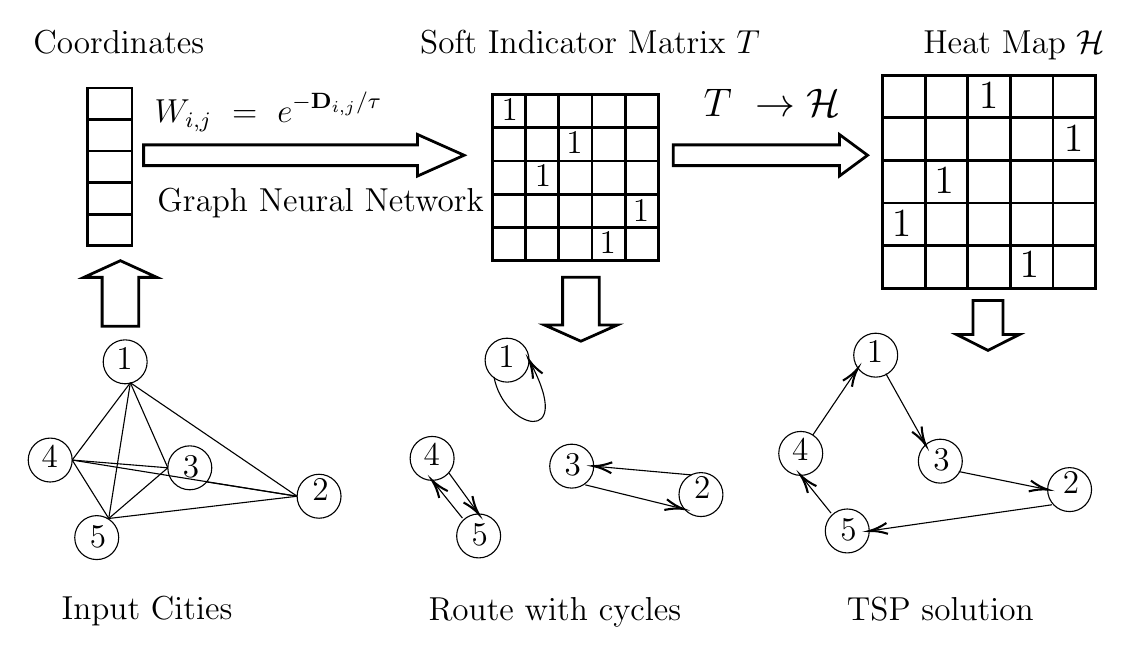
\begin{tikzpicture}[x=0.6pt,y=0.6pt,yscale=-1,xscale=1]
%uncomment if require: \path (0,387); %set diagram left start at 0, and has height of 387

%Shape: Rectangle [id:dp23178493873377803] 
\draw [line width=1.0]  (60,48) -- (87,48) -- (87,67) -- (60,67) -- cycle ;
%Shape: Rectangle [id:dp4704569441411405] 
\draw  [line width=1.0] (60,67) -- (87,67) -- (87,86) -- (60,86) -- cycle ;
%Shape: Rectangle [id:dp25753239564099806] 
\draw  [line width=1.0] (60,86) -- (87,86) -- (87,105) -- (60,105) -- cycle ;
%Shape: Rectangle [id:dp3907839676833267] 
\draw [line width=1.0] (60,105) -- (87,105) -- (87,124) -- (60,124) -- cycle ;
%Shape: Rectangle [id:dp9445302277307268] 
\draw  [line width=1.0] (60,124) -- (87,124) -- (87,143) -- (60,143) -- cycle ;
%Right Arrow [id:dp9781023145195278] 
\draw  [line width=1.0]  (94,82.25) -- (259,82.25) -- (259,76) -- (287,88.5) -- (259,101) -- (259,94.75) -- (94,94.75) -- cycle ;
%Shape: Grid [id:dp0846781272492394] 
\draw  [draw opacity=0][line width=1.]  (304,52) -- (404,52) -- (404,152) -- (304,152) -- cycle ; \draw  [color={rgb, 255:red, 0; green, 0; blue, 0 }  ,draw opacity=1 ][line width=1.]  (324,52) -- (324,152)(344,52) -- (344,152)(364,52) -- (364,152)(384,52) -- (384,152) ; \draw  [color={rgb, 255:red, 0; green, 0; blue, 0 }  ,draw opacity=1 ][line width=1.]  (304,72) -- (404,72)(304,92) -- (404,92)(304,112) -- (404,112)(304,132) -- (404,132) ; \draw  [color={rgb, 255:red, 0; green, 0; blue, 0 }  ,draw opacity=1 ][line width=1]  (304,52) -- (404,52) -- (404,152) -- (304,152) -- cycle ;
%Flowchart: Connector [id:dp5621714533214365] 
\draw   (299.65,211.9) .. controls (299.65,204.59) and (305.57,198.67) .. (312.88,198.67) .. controls (320.19,198.67) and (326.12,204.59) .. (326.12,211.9) .. controls (326.12,219.21) and (320.19,225.13) .. (312.88,225.13) .. controls (305.57,225.13) and (299.65,219.21) .. (299.65,211.9) -- cycle ;
%Flowchart: Connector [id:dp8785665347367976] 
\draw   (254.5,271.06) .. controls (254.5,263.75) and (260.42,257.83) .. (267.73,257.83) .. controls (275.04,257.83) and (280.97,263.75) .. (280.97,271.06) .. controls (280.97,278.37) and (275.04,284.29) .. (267.73,284.29) .. controls (260.42,284.29) and (254.5,278.37) .. (254.5,271.06) -- cycle ;
%Flowchart: Connector [id:dp38287247752455655] 
\draw   (416.42,292.86) .. controls (416.42,285.55) and (422.34,279.62) .. (429.65,279.62) .. controls (436.96,279.62) and (442.88,285.55) .. (442.88,292.86) .. controls (442.88,300.17) and (436.96,306.09) .. (429.65,306.09) .. controls (422.34,306.09) and (416.42,300.17) .. (416.42,292.86) -- cycle ;
%Flowchart: Connector [id:dp007048724057071243] 
\draw   (282.52,317.77) .. controls (282.52,310.46) and (288.45,304.53) .. (295.76,304.53) .. controls (303.07,304.53) and (308.99,310.46) .. (308.99,317.77) .. controls (308.99,325.08) and (303.07,331) .. (295.76,331) .. controls (288.45,331) and (282.52,325.08) .. (282.52,317.77) -- cycle ;
%Flowchart: Connector [id:dp7442080375309715] 
\draw   (338.57,275.73) .. controls (338.57,268.42) and (344.5,262.5) .. (351.8,262.5) .. controls (359.11,262.5) and (365.04,268.42) .. (365.04,275.73) .. controls (365.04,283.04) and (359.11,288.96) .. (351.8,288.96) .. controls (344.5,288.96) and (338.57,283.04) .. (338.57,275.73) -- cycle ;
%Straight Lines [id:da23177368081511884] 
\draw    (424,281.02) -- (367.03,275.91) ;
\draw [shift={(365.04,275.73)}, rotate = 5.12] [color={rgb, 255:red, 0; green, 0; blue, 0 }  ][line width=0.75]    (10.93,-3.29) .. controls (6.95,-1.4) and (3.31,-0.3) .. (0,0) .. controls (3.31,0.3) and (6.95,1.4) .. (10.93,3.29)   ;
%Straight Lines [id:da9911712834185168] 
\draw    (359.99,287) -- (417.06,301.04) ;
\draw [shift={(419,301.52)}, rotate = 193.82] [color={rgb, 255:red, 0; green, 0; blue, 0 }  ][line width=0.75]    (10.93,-3.29) .. controls (6.95,-1.4) and (3.31,-0.3) .. (0,0) .. controls (3.31,0.3) and (6.95,1.4) .. (10.93,3.29)   ;
%Straight Lines [id:da21777222933764162] 
\draw    (278,280.02) -- (294.58,302.91) ;
\draw [shift={(295.76,304.53)}, rotate = 234.09] [color={rgb, 255:red, 0; green, 0; blue, 0 }  ][line width=0.75]    (10.93,-3.29) .. controls (6.95,-1.4) and (3.31,-0.3) .. (0,0) .. controls (3.31,0.3) and (6.95,1.4) .. (10.93,3.29)   ;
%Straight Lines [id:da560200327868167] 
\draw    (285.99,307) -- (268.99,285.85) ;
\draw [shift={(267.73,284.29)}, rotate = 51.2] [color={rgb, 255:red, 0; green, 0; blue, 0 }  ][line width=0.75]    (10.93,-3.29) .. controls (6.95,-1.4) and (3.31,-0.3) .. (0,0) .. controls (3.31,0.3) and (6.95,1.4) .. (10.93,3.29)   ;
%Curve Lines [id:da48248842390991165] 
\draw    (305,222.02) .. controls (310.94,253.71) and (354.24,264.68) .. (326.96,213.47) ;
\draw [shift={(326.12,211.9)}, rotate = 61.31] [color={rgb, 255:red, 0; green, 0; blue, 0 }  ][line width=0.75]    (10.93,-3.29) .. controls (6.95,-1.4) and (3.31,-0.3) .. (0,0) .. controls (3.31,0.3) and (6.95,1.4) .. (10.93,3.29)   ;
%Up Arrow [id:dp30236869182171433] 
\draw  [line width=1.0] (58,162.05) -- (80,152) -- (102,162.05) -- (91,162.05) -- (91,191.5) -- (69,191.5) -- (69,162.05) -- cycle ;
%Flowchart: Connector [id:dp19859424671654013] 
\draw   (69.65,212.9) .. controls (69.65,205.59) and (75.57,199.67) .. (82.88,199.67) .. controls (90.19,199.67) and (96.12,205.59) .. (96.12,212.9) .. controls (96.12,220.21) and (90.19,226.13) .. (82.88,226.13) .. controls (75.57,226.13) and (69.65,220.21) .. (69.65,212.9) -- cycle ;
%Flowchart: Connector [id:dp14897267944646286] 
\draw   (24.5,272.06) .. controls (24.5,264.75) and (30.42,258.83) .. (37.73,258.83) .. controls (45.04,258.83) and (50.97,264.75) .. (50.97,272.06) .. controls (50.97,279.37) and (45.04,285.29) .. (37.73,285.29) .. controls (30.42,285.29) and (24.5,279.37) .. (24.5,272.06) -- cycle ;
%Flowchart: Connector [id:dp6534623508391503] 
\draw   (186.42,293.86) .. controls (186.42,286.55) and (192.34,280.62) .. (199.65,280.62) .. controls (206.96,280.62) and (212.88,286.55) .. (212.88,293.86) .. controls (212.88,301.17) and (206.96,307.09) .. (199.65,307.09) .. controls (192.34,307.09) and (186.42,301.17) .. (186.42,293.86) -- cycle ;
%Flowchart: Connector [id:dp08186289142508718] 
\draw   (52.52,318.77) .. controls (52.52,311.46) and (58.45,305.53) .. (65.76,305.53) .. controls (73.07,305.53) and (78.99,311.46) .. (78.99,318.77) .. controls (78.99,326.08) and (73.07,332) .. (65.76,332) .. controls (58.45,332) and (52.52,326.08) .. (52.52,318.77) -- cycle ;
%Straight Lines [id:da10237177908278228] 
\draw    (108.57,276.73) -- (86,225.5) ;
%Straight Lines [id:da4375992701769358] 
\draw    (132,285.25) -- (186.42,293.86) ;
%Straight Lines [id:da25285152712395553] 
\draw    (86,225.5) -- (186.42,293.86) ;
%Straight Lines [id:da6532543372591861] 
\draw    (73,307.25) -- (186.42,293.86) ;
%Straight Lines [id:da1258686687479621] 
\draw    (50.97,272.06) -- (186.42,293.86) ;
%Straight Lines [id:da8067753221067242] 
\draw    (73,307.25) -- (108.57,276.73) ;
%Straight Lines [id:da974170210303272] 
\draw    (73,307.25) -- (86,225.5) ;
%Straight Lines [id:da9221039867973873] 
\draw    (50.97,272.06) -- (86,225.5) ;
%Straight Lines [id:da26726764184579] 
\draw    (73,307.25) -- (50.97,272.06) ;
%Straight Lines [id:da6861864197145535] 
\draw    (108.57,276.73) -- (50.97,272.06) ;
%Up Arrow [id:dp9044125341581671] 
\draw  [line width=1.0]  (379.33,190.7) -- (357.33,200.5) -- (335.33,190.7) -- (346.33,190.7) -- (346.33,162) -- (368.33,162) -- (368.33,190.7) -- cycle ;
%Right Arrow [id:dp6531154599230456] 
\draw  [line width=1.0]  (413,82.25) -- (513.03,82.25) -- (513.03,76) -- (530,88.5) -- (513.03,101) -- (513.03,94.75) -- (413,94.75) -- cycle ;
%Shape: Grid [id:dp6620827806240519] 
\draw  [draw opacity=0][line width=1.0]  (539,40.28) -- (667.36,40.28) -- (667.36,168.64) -- (539,168.64) -- cycle ; \draw  [color={rgb, 255:red, 0; green, 0; blue, 0 }  ,draw opacity=1 ][line width=1.0]  (564.67,40.28) -- (564.67,168.64)(590.34,40.28) -- (590.34,168.64)(616.01,40.28) -- (616.01,168.64)(641.69,40.28) -- (641.69,168.64) ; \draw  [color={rgb, 255:red, 0; green, 0; blue, 0 }  ,draw opacity=1 ][line width=1.0]  (539,65.96) -- (667.36,65.96)(539,91.63) -- (667.36,91.63)(539,117.3) -- (667.36,117.3)(539,142.97) -- (667.36,142.97) ; \draw  [color={rgb, 255:red, 0; green, 0; blue, 0 }  ,draw opacity=1 ][line width=1.0]  (539,40.28) -- (667.36,40.28) -- (667.36,168.64) -- (539,168.64) -- cycle ;
%Down Arrow [id:dp3866174715686681] 
\draw [line width=1.0]   (621.5,196.43) -- (602.5,206) -- (583.5,196.43) -- (593.5,196.43) -- (593.5,176) -- (611.5,176) -- (611.5,196.43) -- cycle ;
%Flowchart: Connector [id:dp5109060170262866] 
\draw  (521.65,208.9) .. controls (521.65,201.59) and (527.57,195.67) .. (534.88,195.67) .. controls (542.19,195.67) and (548.12,201.59) .. (548.12,208.9) .. controls (548.12,216.21) and (542.19,222.13) .. (534.88,222.13) .. controls (527.57,222.13) and (521.65,216.21) .. (521.65,208.9) -- cycle ;
%Flowchart: Connector [id:dp9913622859051902] 
\draw   (476.5,268.06) .. controls (476.5,260.75) and (482.42,254.83) .. (489.73,254.83) .. controls (497.04,254.83) and (502.97,260.75) .. (502.97,268.06) .. controls (502.97,275.37) and (497.04,281.29) .. (489.73,281.29) .. controls (482.42,281.29) and (476.5,275.37) .. (476.5,268.06) -- cycle ;
%Flowchart: Connector [id:dp411659662460367] 
\draw   (638.42,289.86) .. controls (638.42,282.55) and (644.34,276.62) .. (651.65,276.62) .. controls (658.96,276.62) and (664.88,282.55) .. (664.88,289.86) .. controls (664.88,297.17) and (658.96,303.09) .. (651.65,303.09) .. controls (644.34,303.09) and (638.42,297.17) .. (638.42,289.86) -- cycle ;
%Flowchart: Connector [id:dp3084218640266059] 
\draw   (504.52,314.77) .. controls (504.52,307.46) and (510.45,301.53) .. (517.76,301.53) .. controls (525.07,301.53) and (530.99,307.46) .. (530.99,314.77) .. controls (530.99,322.08) and (525.07,328) .. (517.76,328) .. controls (510.45,328) and (504.52,322.08) .. (504.52,314.77) -- cycle ;
%Flowchart: Connector [id:dp3768575344941739] 
\draw   (560.57,272.73) .. controls (560.57,265.42) and (566.5,259.5) .. (573.8,259.5) .. controls (581.11,259.5) and (587.04,265.42) .. (587.04,272.73) .. controls (587.04,280.04) and (581.11,285.96) .. (573.8,285.96) .. controls (566.5,285.96) and (560.57,280.04) .. (560.57,272.73) -- cycle ;
%Straight Lines [id:da20228889797782246] 
\draw    (540.99,220) -- (564.02,261.25) ;
\draw [shift={(564.99,263)}, rotate = 240.83] [color={rgb, 255:red, 0; green, 0; blue, 0 }  ][line width=0.75]    (10.93,-3.29) .. controls (6.95,-1.4) and (3.31,-0.3) .. (0,0) .. controls (3.31,0.3) and (6.95,1.4) .. (10.93,3.29)   ;
%Straight Lines [id:da1986778844098568] 
\draw    (584.99,279) -- (636.46,289.46) ;
\draw [shift={(638.42,289.86)}, rotate = 191.49] [color={rgb, 255:red, 0; green, 0; blue, 0 }  ][line width=0.75]    (10.93,-3.29) .. controls (6.95,-1.4) and (3.31,-0.3) .. (0,0) .. controls (3.31,0.3) and (6.95,1.4) .. (10.93,3.29)   ;
%Straight Lines [id:da13868326492774685] 
\draw    (640.99,299) -- (552.17,311.73) -- (532.97,314.48) ;
\draw [shift={(530.99,314.77)}, rotate = 351.84] [color={rgb, 255:red, 0; green, 0; blue, 0 }  ][line width=0.75]    (10.93,-3.29) .. controls (6.95,-1.4) and (3.31,-0.3) .. (0,0) .. controls (3.31,0.3) and (6.95,1.4) .. (10.93,3.29)   ;
%Straight Lines [id:da4310681916397241] 
\draw    (507.99,304) -- (490.99,282.85) ;
\draw [shift={(489.73,281.29)}, rotate = 51.2] [color={rgb, 255:red, 0; green, 0; blue, 0 }  ][line width=0.75]    (10.93,-3.29) .. controls (6.95,-1.4) and (3.31,-0.3) .. (0,0) .. controls (3.31,0.3) and (6.95,1.4) .. (10.93,3.29)   ;
%Straight Lines [id:da14237151872316922] 
\draw    (496.99,257) -- (522.87,218.66) ;
\draw [shift={(523.99,217)}, rotate = 124.02] [color={rgb, 255:red, 0; green, 0; blue, 0 }  ][line width=0.75]    (10.93,-3.29) .. controls (6.95,-1.4) and (3.31,-0.3) .. (0,0) .. controls (3.31,0.3) and (6.95,1.4) .. (10.93,3.29)   ;
%Flowchart: Connector [id:dp9287080412224115] 
\draw   (108.57,276.73) .. controls (108.57,269.42) and (114.5,263.5) .. (121.8,263.5) .. controls (129.11,263.5) and (135.04,269.42) .. (135.04,276.73) .. controls (135.04,284.04) and (129.11,289.96) .. (121.8,289.96) .. controls (114.5,289.96) and (108.57,284.04) .. (108.57,276.73) -- cycle ;

% Text Node
\draw (26,12) node [anchor=north west][inner sep=0.75pt]  [font=\large] [align=left] {Coordinates};
% Text Node
\draw (99,49) node [anchor=north west][inner sep=0.75pt]   [align=left] {{\large $\displaystyle W_{i,j} \ =\ e^{ -\mathbf{D}_{i,j} /\tau }$}};
% Text Node
\draw (101,107) node [anchor=north west][inner sep=0.6pt] [font=\large]   [align=left] {Graph Neural Network};
% \draw (101,107) node [anchor=north west][inner sep=0.6pt]   [align=left] {{$\displaystyle \begin{array}{{>{\displaystyle}l}}
% Scattering\ Attention\ \\
% Graph\ Neural\ Network
% \end{array}$}};
% Text Node
\draw (259,12) node [anchor=north west][inner sep=0.75pt]  [font=\large] [align=left] {Soft Indicator Matrix $\mathbb{T}$};
% Text Node
\draw (308,53) node [anchor=north west][inner sep=0.75pt]  [font=\large,color={rgb, 255:red, 0; green, 0; blue, 0 }  ,opacity=1 ]
[align=left] {1};
% Text Node
\draw (347,73) node [anchor=north west][inner sep=0.75pt]  [font=\large,color={rgb, 255:red, 0; green, 0; blue, 0 }  ,opacity=1 ] [align=left] {1};
% Text Node
\draw (328,93) node [anchor=north west][inner sep=0.75pt]  [font=\large,color={rgb, 255:red, 0; green, 0; blue, 0 }  ,opacity=1 ][align=left] {1};
% Text Node
\draw (387,114) node [anchor=north west][inner sep=0.75pt]  [font=\large,color={rgb, 255:red, 0; green, 0; blue, 0 }  ,opacity=1 ][align=left] {1};
% Text Node
\draw (367,133) node [anchor=north west][inner sep=0.75pt]  [font=\large,color={rgb, 255:red, 0; green, 0; blue, 0 }  ,opacity=1 ][align=left] {1};
% Text Node
\draw (306,202) node [anchor=north west][inner sep=0.75pt]   [align=left] {{\large 1}};
% Text Node
\draw (424,281) node [anchor=north west][inner sep=0.75pt]   [align=left] {{\large 2}};
% Text Node
\draw (346,267) node [anchor=north west][inner sep=0.75pt]   [align=left] {{\large 3}};
% Text Node
\draw (261,261) node [anchor=north west][inner sep=0.75pt]   [align=left] {{\large 4}};
% Text Node
\draw (290,309) node [anchor=north west][inner sep=0.75pt]   [align=left] {{\large 5}};
% Text Node
\draw (264,353) node [anchor=north west][inner sep=0.75pt]   [align=left] {{\large Route with cycles}};
% Text Node
\draw (76,203) node [anchor=north west][inner sep=0.75pt]   [align=left] {{\large 1}};
% Text Node
\draw (194,282) node [anchor=north west][inner sep=0.75pt]   [align=left] {{\large 2}};
% Text Node
\draw  (116,268) node [anchor=north west][inner sep=0.75pt]   [align=left] {{\large 3}};
% Text Node
\draw (31,262) node [anchor=north west][inner sep=0.75pt]   [align=left] {{\large 4}};
% Text Node
\draw (60,310) node [anchor=north west][inner sep=0.75pt]   [align=left] {{\large 5}};
% Text Node
\draw (429.67,47.07) node [anchor=north west][inner sep=0.75pt]  [font=\Large]  {$\mathbb{T} \ \rightarrow \mathcal{H}$};
% Text Node
\draw (43,353) node [anchor=north west][inner sep=0.75pt]   [align=left] {{\large Input Cities}};
% Text Node
\draw (595.46,43.54) node [anchor=north west][inner sep=0.75pt]  [font=\large,color={rgb, 255:red, 0; green, 0; blue, 0 }  ,opacity=1 ] [align=left] {{\Large 1}};
% Text Node
\draw (646.69,68.96) node [anchor=north west][inner sep=0.75pt]  [font=\large,color={rgb, 255:red, 0; green, 0; blue, 0 }  ,opacity=1 ] [align=left] {{\Large 1}};
% Text Node
\draw (568.67,94.63) node [anchor=north west][inner sep=0.75pt]  [font=\large,color={rgb, 255:red, 0; green, 0; blue, 0 }  ,opacity=1 ] [align=left] {{\Large 1}};
% Text Node
\draw (543,120.3) node [anchor=north west][inner sep=0.75pt]  [font=\large,color={rgb, 255:red, 0; green, 0; blue, 0 }  ,opacity=1 ] [align=left] {{\Large 1}};
% Text Node
\draw (620.01,144.97) node [anchor=north west][inner sep=0.75pt]  [font=\large,color={rgb, 255:red, 0; green, 0; blue, 0 }  ,opacity=1 ] [align=left] {{\Large 1}};
% Text Node
\draw (562,12) node [anchor=north west][inner sep=0.75pt]  [font=\large] [align=left] {Heat Map $\mathcal{H}$};
% Text Node
\draw (528,199) node [anchor=north west][inner sep=0.75pt]   [align=left] {{\large 1}};
% Text Node
\draw (646,278) node [anchor=north west][inner sep=0.75pt]   [align=left] {{\large 2}};
% Text Node
\draw (568,264) node [anchor=north west][inner sep=0.75pt]   [align=left] {{\large 3}};
% Text Node
\draw (483,258) node [anchor=north west][inner sep=0.75pt]   [align=left] {{\large 4}};
% Text Node
\draw (512,306) node [anchor=north west][inner sep=0.75pt]   [align=left] {{\large 5}};
% Text Node
\draw (516,353) node [anchor=north west][inner sep=0.75pt]   [align=left] {{\large TSP solution}};
\end{tikzpicture}
\caption{We use a SAG to generate a non-smooth soft indicator matrix $\mathbb{T}$. The SAG model is a function of  coordinates and weighted adjacency matrix. We then build the heat map $\mathcal{H}$ based on $\mathbb{T}$ using the transformation in Equation ~\ref{eq:TH}. }
\label{fig:TSP}
\end{figure}

To better understand the $\mathbb{T} \rightarrow \mathcal{H}$ transformation, we show a binary instance in Figure~\ref{fig:TSP}. Figure~\ref{fig:TSP} illustrates a soft indicator matrix $\mathbb{T}$, its heat map  $\mathcal{H}$ following the transformation $\mathbb{T} \rightarrow \mathcal{H}$, and their corresponding routes. When we directly use the soft indicator matrix $\mathbb{T}$ as the heat map. It can result in loops (parallel edges) between cities, such as  (2,3) and (4,5) in Figure~\ref{fig:TSP} (middle). After we apply the $\mathbb{T} \rightarrow \mathcal{H}$  transformation, the corresponding heat $\mathcal{H}$ is a Hamiltonian Cycle, as shown in the right part in Figure~\ref{fig:TSP}. 

\subsection{$\mathbb{T} \rightarrow \mathcal{H}$  transformation}
We build the heat map $\mathcal{H}$ based on $\mathbb{T}$. As mentioned, $\mathcal{H}_{i,j}$ is the probability for edge ($i$,$j$) to belong to the optimal TSP solution. We define $\mathcal{H}$ as:
\begin{equation}\label{eq:TH}
\mathcal{H} = \sum_{t=1}^{n-1}p_t p^T_{t+1} + p_np_1^T,
\end{equation}
where $p_t \in \mathbb{R}^{n \times 1}$ is the $t_{th}$ column of $\mathbb{T}$, $\mathbb{T} = [p_1|p_2|...|p_n]$.
% The elements in $\mathcal{H}$ can be written as
As shown in Figure~\ref{fig:TSP}, the first row in $\mathcal{H}$ is the probability distribution of directed edges start from city $1$, and since the third element is the only non-zero one in the first row, we then add directed edge $1 \rightarrow 3 $ to our TSP solution. Similarly, the first column in $\mathcal{H}$ can be regarded as the probability distribution of directed edges which end in city $1$.  Ideally, given a graph $\mathcal{G}$ with $n$ nodes, we want to build a soft indicator matrix where  each row and column are assigned with one value 1 (True) and $n-1$ values 0 (False), so that the heat map will only contain one valid solution. 
% Equation~\ref{eq:Hij} generate a Hamiltonian Cycle given $\mathbb{T}$. 
In practice, we will build a soft indicator matrix $\mathbb{T}$ whose heat map $\mathcal{H}$ assigns large probabilities to the edges in the TSP solution and small probabilities to the other edges.


Overall, the $\mathbb{T} \rightarrow \mathcal{H}$ transformation in Equation~\ref{eq:TH} enables us to build a proxy for the Hamiltonian Cycle constraint. We further prove that $\mathcal{H}$ represents one Hamiltonian Cycle when each row and column in  $\mathbb{T} $ have one value 1 (True) and $n-1$ value 0 (False). We refer to the proof in  appendix~\ref{sec:proof}. 

\subsection{Unsupervised Loss}
In order to generate such an expressive soft indicator matrix $\mathbb{T}$, we minimize the following objective function:
\begin{equation} \label{eq:loss}
\begin{aligned}
    \mathcal{L} =   
 \lambda_1 \underbrace{\sum_{i=1}^n (\sum_{j=1}^n \mathbb{T}_{i,j} - 1)^2}_{\text{Row-wise constraint}}  +  \lambda_2   \underbrace{\sum_{i}^n \mathcal{H}_{i,i}}_{\text{No self-loops}}  + \underbrace{\sum_{i=1}^n \sum_{j=1}^n \mathbf{D}_{i,j} \mathcal{H}_{i,j}}_{\text{Minimize the distance }}. 
\end{aligned}
\end{equation}

The first term in $\mathcal{L}$ encourages the summation of each row in $\mathbb{T}$ to be close to 1. As mentioned, we normalize each column of $\mathbb{T}$ using  Softmax activation. So when the first term is minimized to zero, each row and column in $\mathbb{T}$ are normalized (doubly stochastic). The second term penalizes the weight on the main diagonal of $\mathcal{H}$, this discourages self-loops in  TSP solutions. The third term can be regarded as the expected TSP length of the heat map $\mathcal{H}$, where $\mathbf{D}_{i,j}$ is the distance between city $i$ and $j$. As mentioned, since $\mathcal{H}$ corresponds to a Hamiltonian Cycle given an ideal soft indicator matrix with one value $1$ (True)
and $n-1$ value $0$ (False) in each row and column. Then the minimum value of $\sum_{i=1}^n \sum_{j=1}^n \mathbf{D}_{i,j} \mathcal{H}_{i,j}$ is the shortest Hamiltonian Cycle on the graph, which is the optimal solution of TSP. To summarize, we build a loss function which contains both the \textit{shortest} and the \textit{Hamiltonian Cycle} constraints. The \textit{shortest} constraint is realized by minimizing 
$
\sum_{i=1}^n \sum_{j=1}^n \mathbf{D}_{i,j} \mathcal{H}_{i,j}.
$
For the \textit{Hamiltonian Cycle} constraint, instead of writing it in a Lagrangian relaxation style penalty, we use a GNN which encourages a non-smooth representation, along with the doubly stochastic penalty, and the $\mathbb{T}\rightarrow \mathcal{H}$ transformation.

\subsection{Edge Elimination} Given a heat map $\mathcal{H}$, we consider  $M$ largest elements in each row (without diagonal elements) and set other $n-M$ %(\Yiwei{Can we replace K with M here for later consistency}) 
elements as 0. Let $\Tilde{H}$ denote the new heat map, we then symmetrize the new heat map by $\mathcal{H}' = \Tilde{H} + \Tilde{H}^T$. %because the reverse of a Hamiltonian Cycle is also a Hamiltonian Cycle. 
Let $\mathbf{E}_{ij} \in \{0,1\}$ denote whether an undirected edge ($i,j$)  is in our prediction or not. Without loss of generality, we can assume $0<i<j\leq n$ and  define $\mathbf{E}_{ij}$ as :
$$
\mathbf{E}_{ij} = 
    \begin{cases}
      1, & \text{if}\ \mathcal{H}'_{ij} = \mathcal{H}'_{ji} > 0 \\
      0, & \text{otherwise}
    \end{cases}.
$$
Let $\Pi$ denote the set of undirected edges $(i,j)$ with $\mathbf{E}_{ij} = 1$. Ideally, we would build a prediction edge set $\Pi$ with a small $M$ value, and $\Pi$ can cover all the ground truth edges so that we can reduce search space size from $n(n-1)/2$ to  $|\Pi|$. 
% In practice, generating small-size edge sets $\Pi$ which always cover the ground truth solutions is very difficult. 
In practice, we aim to let  $\Pi$ cover as many ground truth edges as possible and use $\mathcal{H}'$ to guide the local search process. 
